The Cox PH is a common approach to analysing time-to-event data \cite{George;2014}. It assumes that the subjects being followed up are at risk of an event (e.g., death). This risk can change over time and it is called "hazard". The hazard then is a function of time which proportionately changes with covariates. For example, consider a study of how tumour size affects survival. For simplicity, say there are two sizes --- large and small. It may be found that large tumours increase the risk of death by 2 as compared to small tumours. This would mean that the hazard for the large-tumour group is twice the hazard for the small-tumour group at any time.

For the Cox PH regression, the outcome is time-to-event. This time should normally be time at risk of an observable event. As an illustration, in Figure \ref{CoxExampleFull}, two subjects are followed until both experience an event (e.g., infection).

\begin{figure}[htp]
	\centering
	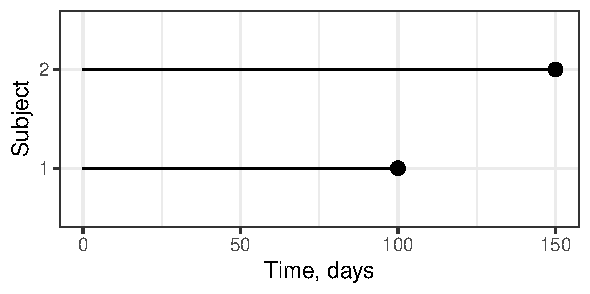
\includegraphics[width=0.6\textwidth]{../curve-cox/timeplot_1_light.pdf}
	\caption{
	An example of time-to-event data. Two subjects are followed from time 0. Subject 1 experiences the even at time 100. Subject 2 experiences the event at time 150.
	}
	\label{CoxExampleFull}
\end{figure}

Since subject 2 experienced the event later (i.e., ``survived'' for longer), the covariate pattern (e.g., antibody titre) of subject 2 would be considered by the model to be more ``protective'' than that of subject 1. That is, their covariates would be consistent with a reduced hazard. For the purposes of this discussion, we will assume that a subject can only experience one event after which they are no longer at risk for the remainder of the follow-up time. For seasonal infectious diseases this may be a reasonable assumption if the follow-up is confined to one season and infection grants immunity for the rest of the season (or is fatal).

If subjects are not at risk for all of their follow-up time (e.g., not exposed to the virus), then the total follow-up time may be misleading as illustrated in Figure \ref{CoxExamplePartial}. Taking the actual time at risk into account would lead to the opposite conclusion in this example --- it is subject 1 who is more ``protected'' since they were at risk for longer.

\begin{figure}[htp]
	\centering
	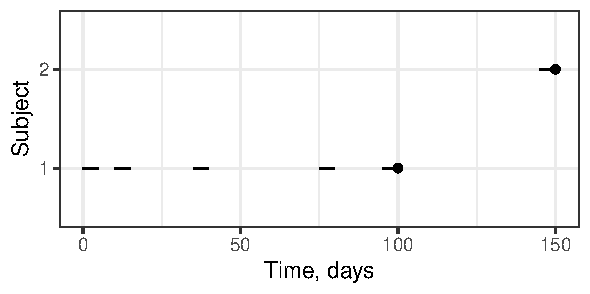
\includegraphics[width=0.6\textwidth]{../curve-cox/timeplot_2_light.pdf}
	\caption{
	An example of time-to-event data. Two subjects are followed from time 0. Subject 1 experiences the even at time 100. Subject 2 experiences the event at time 150. Subject 1 was at risk of the event for a total of 5 days. Subject 2 was at risk of the event for a total of 25 days.
	}
	\label{CoxExamplePartial}
\end{figure}

In infection data, true time at risk is unobservable because the risk of infection among susceptible individuals depends on exposure to the pathogen, which cannot be measured. If follow-up time is completely unrepresentative of true time at risk, the Cox model will not produce meaningful results. However, if the total time of follow-up is assumed to be, on average, proportional to the total time at risk (e.g., subjects who are followed up for longer can be expected to have been exposed for longer) then the situation illustrated in Figure  \ref{CoxExamplePartial} will be ``averaged out'' and the model may still produce meaningful results.

To investigate the behaviour of the estimates when time of follow-up is not the same as time at risk but is proportional to it, we generated a simulated dataset, based on the following model:

\begin{align*}
\begin{gathered}
T \sim \text{Exponential}(\text{rate} = \lambda) \\
h(t) = \lambda \\
\text{log}\lambda = -3 - 1.5 X_{\text{logtitre}}
\end{gathered}
\end{align*}

Where $T$ is the survival time, $h$ is the hazard function and $X_{\text{logtitre}}$ is the true log-titre measurement simulated from $N(2, 2^2)$.

Maximum time of follow-up was set to 100 days. Each individual was assigned a proportion of the follow-up time they were exposed to the virus (time-at-risk proportion). This proportion was generated from $\text{Beta}(\mu \kappa, (1 - \mu) \kappa)$ where $\mu$ is the expected proportion for the population and $\kappa$ is inversely proportional to the variance of the proportion. Smaller $\kappa$ values result in larger heterogeneity of exposure in the population. When $\mu = 1$, the proportion assigned was always 1 to represent the ideal context of all follow-up time being time at risk. An individual's follow-up time was 100 times their time-at-risk proportion.

A random number generated for each individual by $\text{Exponential}(\text{rate} = \text{exp}(-3 - 1.5 X_{\text{logtitre}}) )$ represented the time it would take that individual to experience the event (get infected), that is "survival" time. If survival time was greater than time at risk, the individual was "not infected" and their follow-up time was 100 (i.e., this was a right-censored observation). If survival time was smaller than time at risk, the individual was "infected" and their follow-up time was their survival time divided by their time-at-risk proportion.

Each simulation included 10,000 observations and was run 10,000 times at each of the following values of $\mu$: 0.01, 0.1, 0.2, 0.3, 0.4, 0.5, 0.6, 0.7, 0.9, 1 and at each of the following values of $\kappa$: 0.5, 1, 10, 100, 1000. The Cox proportional hazards model was fit to each simulated dataset. From 10,000 simulations at each combination of values of $\mu$ and $\kappa$, the mean of the estimated coefficient and its standard deviation were saved. The results are summarised in Figure \ref{CoxSimResults}.

In the ideal case ($\mu = 1$) the estimate is unbiased and has the smallest error. As the proportion of time at risk decreases, bias is introduced. More bias is introduced when $\kappa$ is small, i.e. when there is a larger amount of heterogeneity of exposure. When exposure is very similar for all members of the population (large $\kappa$), the model estimate has minimal bias across the range of $\mu$.

\begin{figure}[htp]
	\centering
	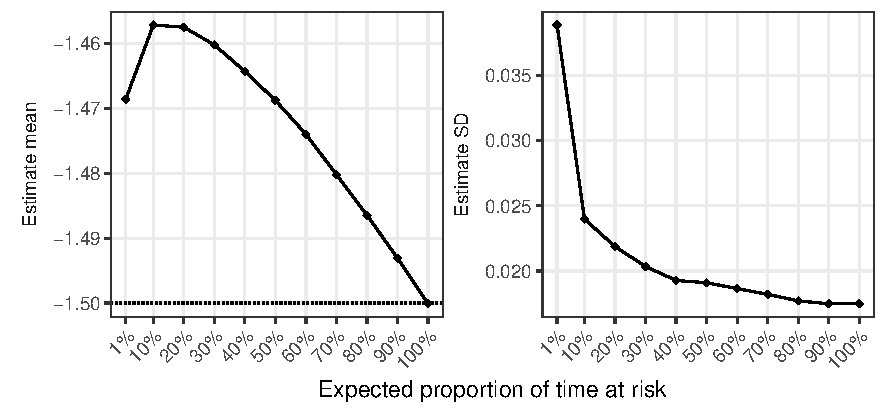
\includegraphics[width=1\textwidth]{../cox-tarprop-plot/risk.pdf}
	\caption{
	The results of fitting a Cox PH model to the time-to-event simulations. For each combination of $\mu$ and $\kappa$, the relative bias of the mean of the estimate (top panel) is shown as well the standard deviation of the estimate (bottom panel) obtained from 10,000 simulations. Points represent the values for which the simulations were performed.
	}
	\label{CoxSimResults}
\end{figure}

The results in Figure \ref{CoxSimResults} show that the Cox PH model can produce (almost) unbiased estimates when time-at-risk is not the same as time-of-follow-up when two assumptions are satisfied. First is that time-at-risk is proportional to time-of-follow-up. Second is that exposure in the population is not overly heterogeneous, e.g. if subjects are expected to have been exposed for 20\% of their follow-up time then each individual subject was exposed for close to 20\% of their follow-up time (corresponds to simulations at $\kappa = 1000,\ \kappa = 100$) rather than having 20\% of the subjects almost always exposed and 80\% almost never exposed (corresponds to simulations at $\kappa = 0.5,\ \kappa = 1$).

The assumption of time at risk being proportional to time of follow-up is likely to hold when everyone in the sample is followed through a period of similar disease activity. There may still be subjects who are not exposed (or over-exposed), but as long as the level of exposure does not correlate with the covariates of interest (e.g., antibody titres), then with a large enough sample size the average exposure for any covariate pattern (e.g., antibody titre level) should be proportional in the same way to the time of follow-up. If the disease is seasonal, the start of follow-up can be set to the start of the season. For those who do not get infected, end of follow-up can then be the end of the season. For those who do get infected, end of follow-up can be the infection time assuming that infection grants immunity for the rest of the season. An illustration is in Figure \ref{CoxIdeal}.

\begin{figure}[htp]
	\centering
	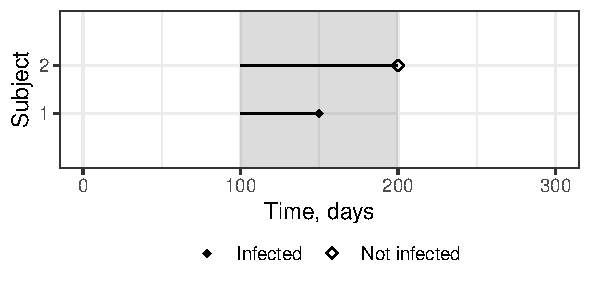
\includegraphics[width=0.59\textwidth]{../curve-cox/timeplot_3_light.pdf}
	\caption{
	An illustration of a pattern of follow-up where the assumption of true time at risk being proportional to time of follow-up is likely to hold. The shaded region marks the period of time when the disease is active. Both subject's follow-up starts at the beginning of the disease season (activity). Subject 1 gets infected at 150 days, their follow-up would end there assuming infection grants immunity (their total recorded time of follow-up would be 50 days). Subject 2 does not get infected through the season, their time of follow-up ends at the end of the season (their total recorded time of follow-up would be 100 days).
	}
	\label{CoxIdeal}
\end{figure}

This assumption will likely not hold if, with a seasonal disease, there are people in the sample whose follow-up starts before the season as shown in Figure \ref{CoxNotIdeal}. For those with earlier follow-up start, their follow-up time will be large regardless of their titres (since they spend a proportion of that time not being at risk). This should make it seem like the titres have a smaller effect than they actually do thus biasing the estimate of titre effect towards the null.

\begin{figure}[htp]
	\centering
	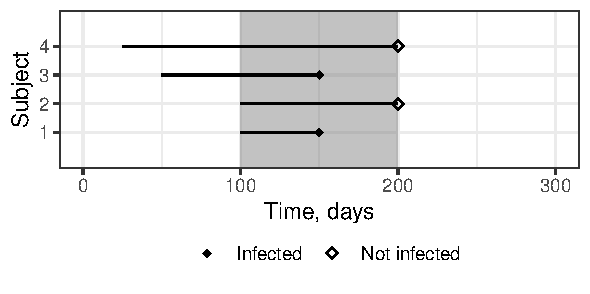
\includegraphics[width=0.59\textwidth]{../curve-cox/timeplot_4_light.pdf}
	\caption{
	An illustration of a pattern of follow-up where the assumption of true time at risk being proportional to time of follow-up is likely to not hold. The shaded region marks the period of time when the disease is active. Subject 1 gets infected at 150 days, at which point their follow-up would end if it can be assumed that infection grants immunity (their total recorded time of follow-up would be 50 days). Subject 2 does not get infected within the season, their follow-up ends at the end of the season (their total recorded time of follow-up would be 100 days). For subjects 3 (recorded follow up of 100 days) and 4 (recorded follow-up of 175 days) follow-up commenced prior to season onset.
	}
	\label{CoxNotIdeal}
\end{figure}

%\pagebreak

To demonstrate this problem, we performed a simulation study using the same procedure as described above, except a proportion of the subjects were randomly chosen to have their follow-up started earlier. For those randomly chosen, a uniform random number between 0 and 200 (days) was added to their recorded follow-up time. The proportion of time at risk was set to 1. The bias resulting from varying the proportion of the sample with earlier follow-up is shown in Figure \ref{CoxSimLong}. The estimate is unbiased when follow-up starts at the start of the season for all subjects. Bias towards the null increases rapidly even when only a small (10\%) proportion of the sample has started follow-up prior to the season. For this reason, it would be advisable to record follow-up time in such a way that true unobservable time at risk can be reasonably expected to be proportional to the recorded time of follow-up (i.e., the longer a subject is followed, the longer they are likely to have been at risk).

\begin{figure}[htp]
	\centering
	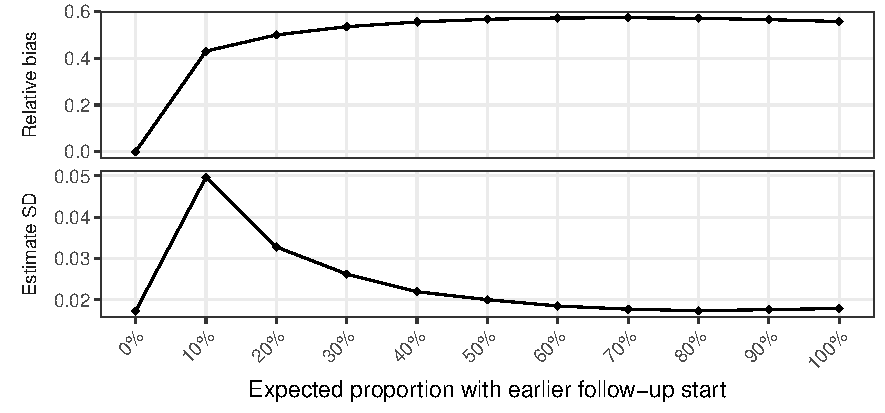
\includegraphics[width=1\textwidth]{../cox-tarprop-plot/long.pdf}
	\caption{
	The results of time-to-event simulations. For each proportion of the sample with earlier follow-up start, the mean of the estimated coefficient (left panel) is shown as well as the standard deviation of that coefficient (right panel) from 10,000 simulations. Points represent the values of expected proportion for which the simulations were performed. The dotted horizontal line is the true value of the estimated parameter.
	}
	\label{CoxSimLong}
\end{figure}
